\section{State of BPMS Solutions}

\begin{figure}[ht!]
	\centering
    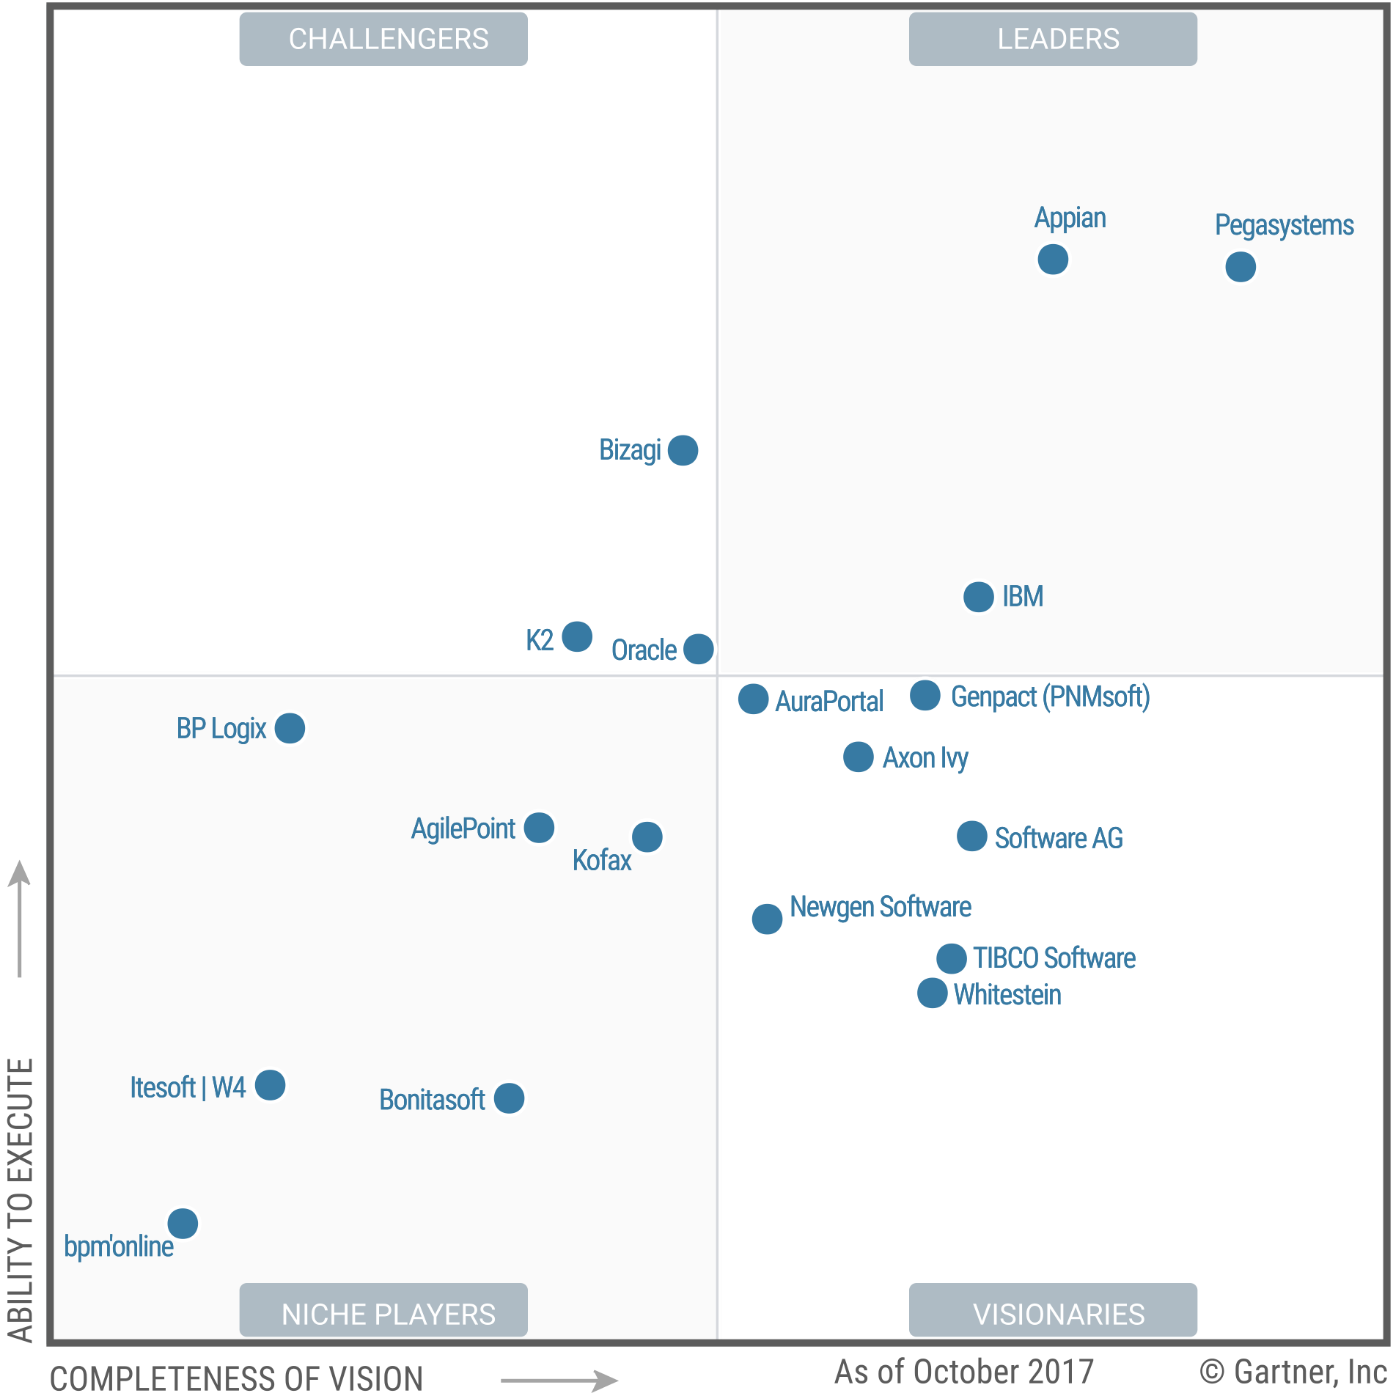
\includegraphics[width=0.6\textwidth, keepaspectratio]{img/gartner-magic-quadrant.png}
    \caption{Gartner Magic Quadrant\cite{gartner-2017} }
    \label{fig:gartner-magic-quadrant}
\end{figure}

Nowadays \gls{bpms} software supports all stages of \gls{bpm} life-cycle (design, modelling, execution, monitoring and optimization). These systems also offer real-time collaboration, integration with cloud and mobile devices. Many systems also integrate artificial intelligence - for predictive analysis or some automatic decisions. \gls{bpms} software allows to create highly productive application, where is no need to manual implementation of business rules. \gls{bpms} includes defining processes, data models and also user interfaces. Also highly customized monitoring stage is included, which means users can customize \gls{kpi} metrics, appearance of dashboard and so on. On top of that functions, some solutions have ability to display (visualise) current running processes.  

Result is typically web based application which employees can use to do their jobs without knowing that there are some defined processes and layer of some BPM software. 

According to \textit{Gartner Magic Quadrant}\cite{gartner-2017}, the most used systems are \textit{Appian}, \textit{Pegasystems}, \textit{IBM} and many more as shown at~\cref{fig:gartner-magic-quadrant}.

 \subsection{Closer Look at Process Maker}
 
 \textit{ProcessMaker} (\href{https://www.processmaker.com/}{https://www.processmaker.com/}) is web-based \gls{bpm} solution which allows to build, run, monitor and optimize business processes. Building of processes is done via \gls{bpmn}. Inside designer %(see \cref{fig:process-maker-designer},
 users can define data sources (variables) which will be used later within running processes. 
 
%  \begin{figure}[ht!]
% 	\centering
%     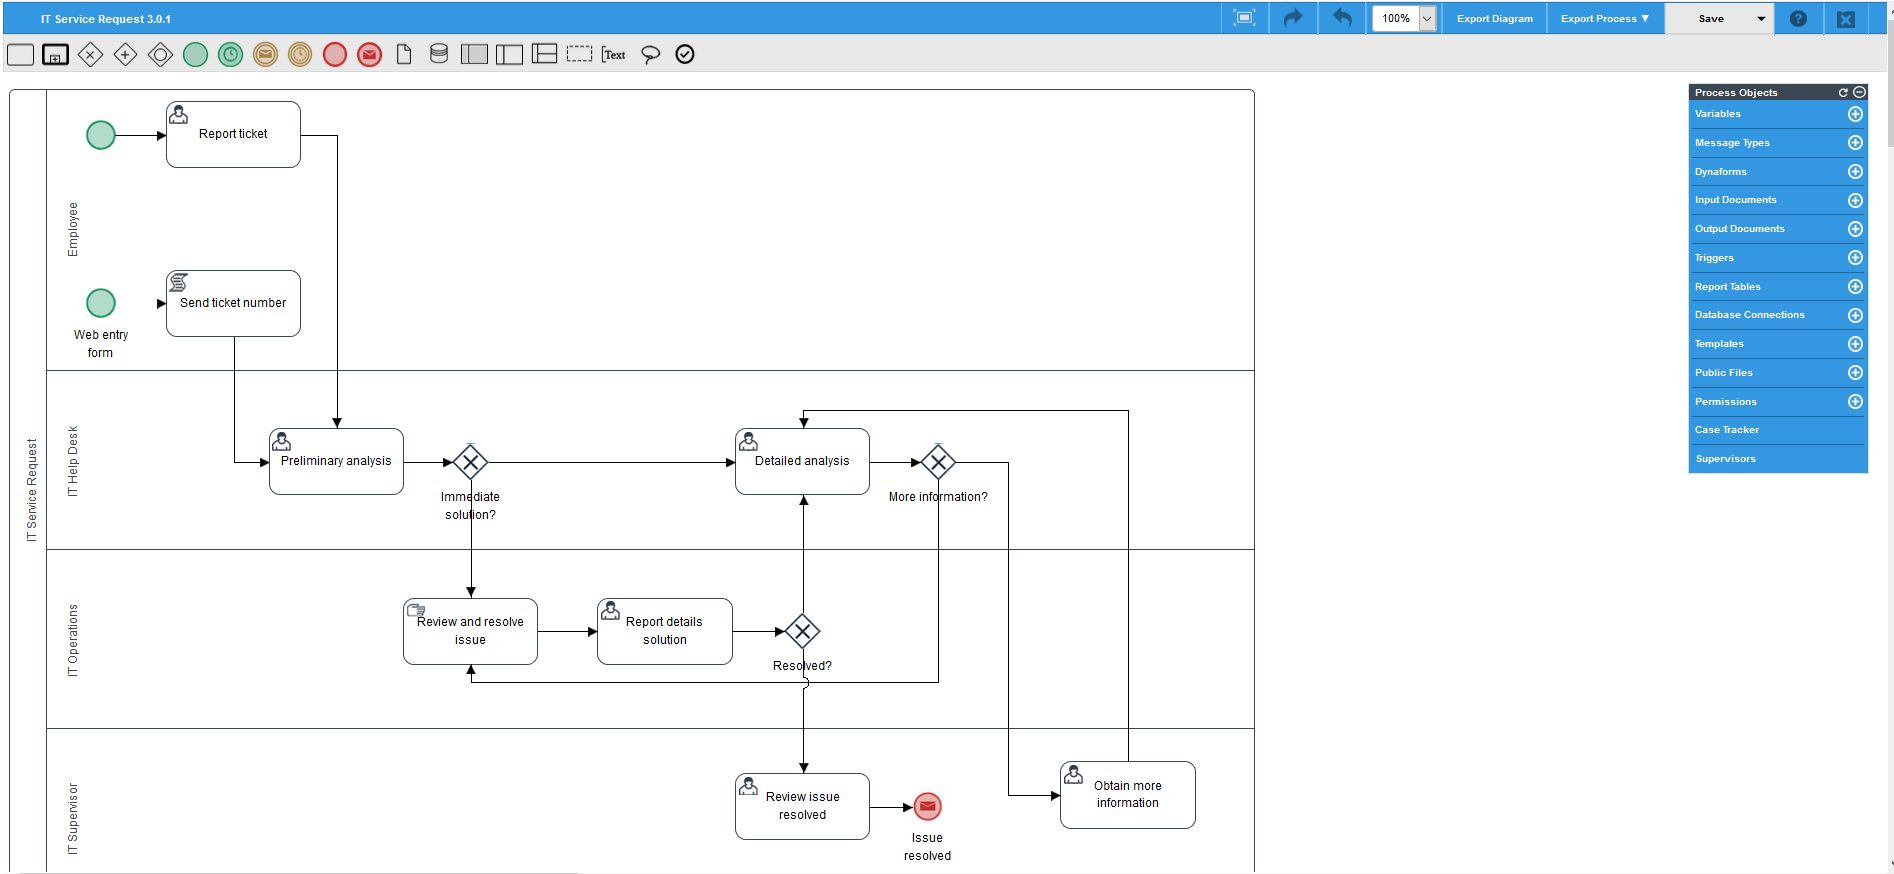
\includegraphics[width=0.8\textwidth, keepaspectratio]{img/process-maker-designer.PNG}
%     \caption{ProcessMaker designer}
%     \label{fig:process-maker-designer}
% \end{figure} 
 
\begin{figure}[ht!]
    \centering
    \subfloat{{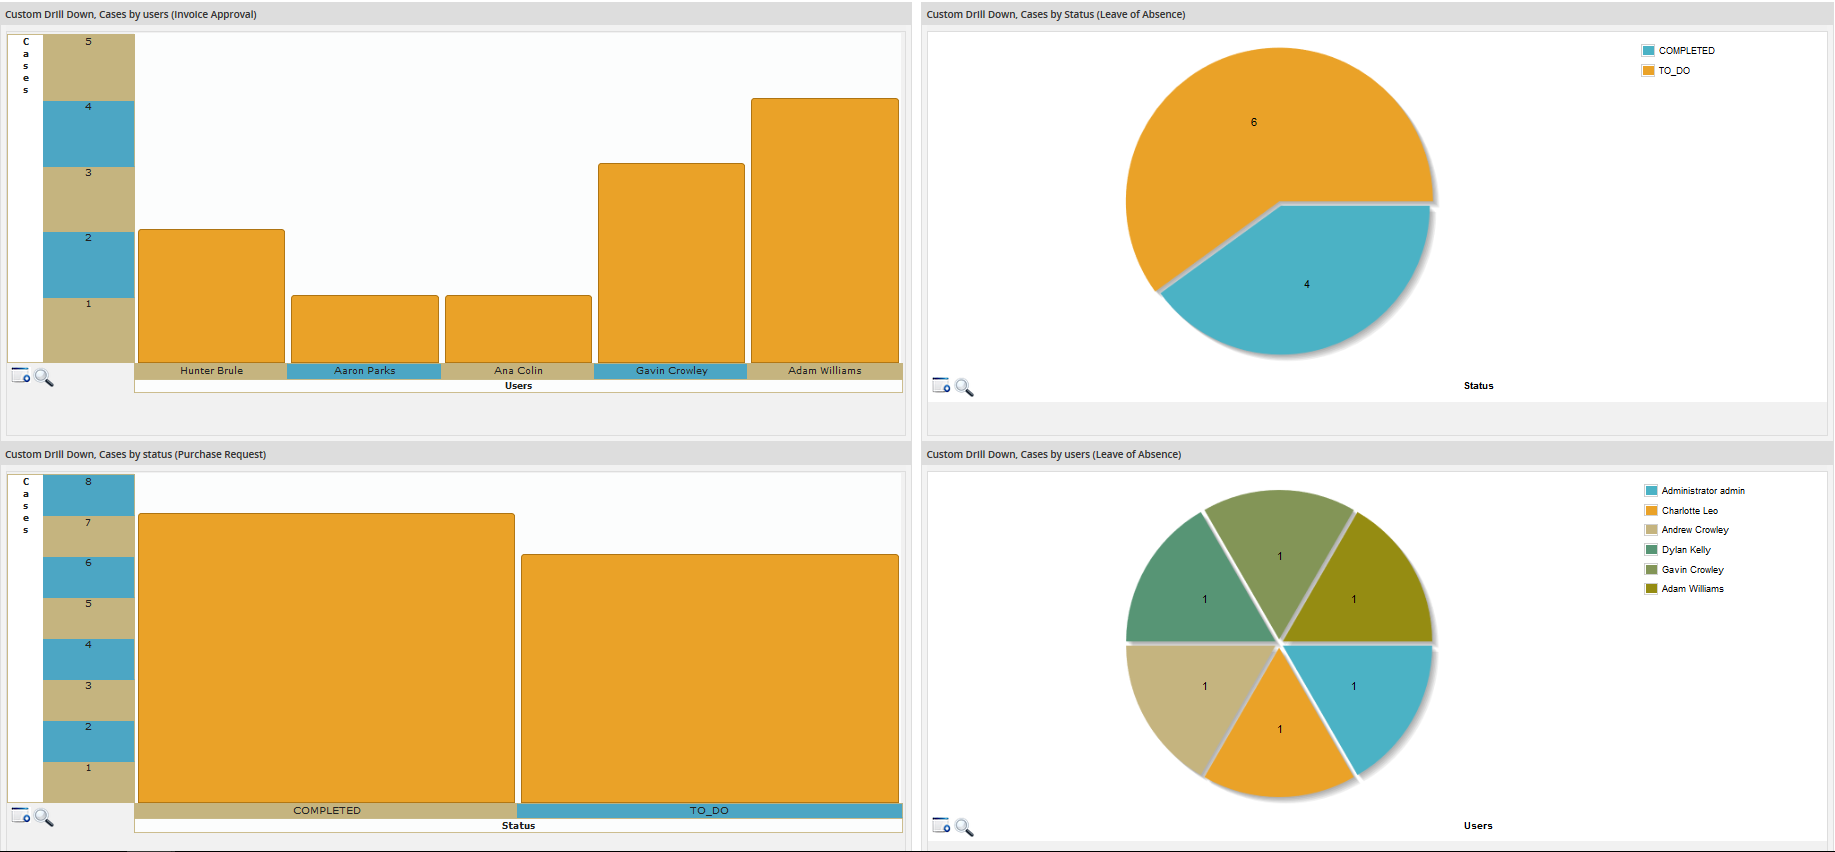
\includegraphics[width=10cm, keepaspectratio]{img/process-maker-dashboard.PNG} }}%
    \qquad
    \subfloat{{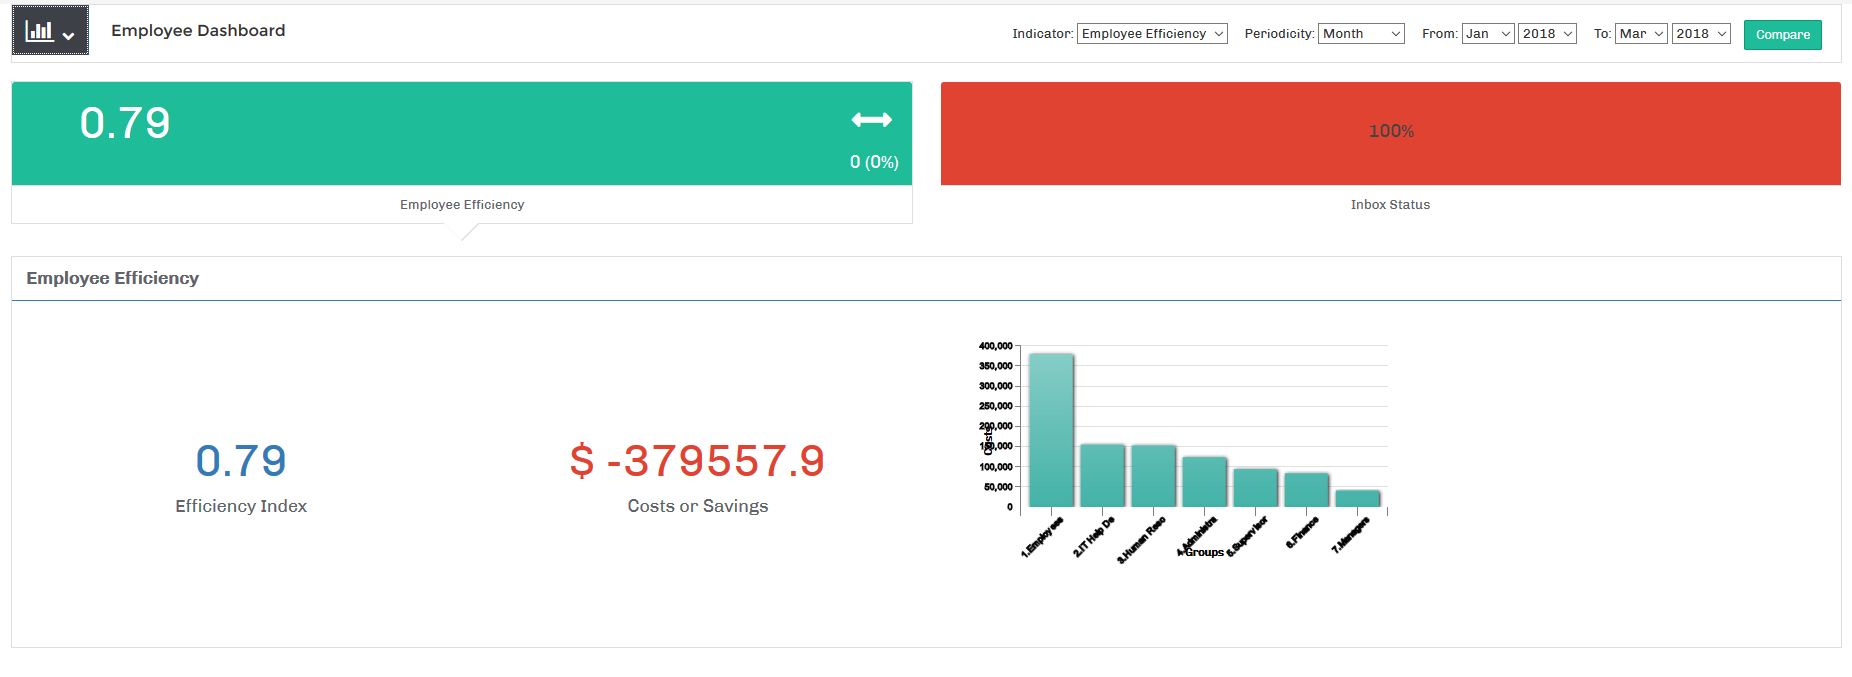
\includegraphics[width=10cm, keepaspectratio]{img/process-maker-employee-kpi.PNG} }}%
    \caption{ProcessMaker dashboard and KPI examples}%
    \label{fig:process-maker-dashboard}%
\end{figure}

 After process is designed and variables defined, next step is to define user interface, called DynaForms. End users interact mainly with \textit{DynaForms}, where they fill appropriate pieces of data. 
 Inside designer of \textit{DynaForms}, user connects data fields with variables from defined processes. Also user can define input or output documents for processes or define events (called triggers) what will happen when some kind of event occurred.
 
 When processes are defined and \textit{DynaForms} created, processes can be deployed. After deploy, \gls{kpi}s and dashboards can be managed. \textit{ProcessMaker} offers creating custom metrics, which will be precise to business requirements and customize dashboards. Many of graphs are interactive, which can display more detailed information. An example is shown at \cref{fig:process-maker-dashboard}.
 
 \begin{figure}[ht!]
	\centering
    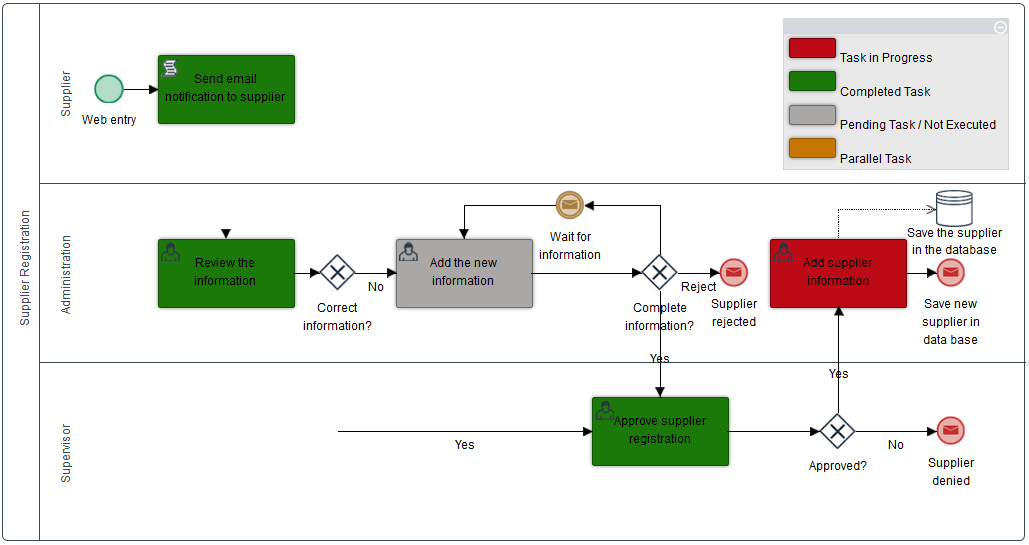
\includegraphics[width=10cm, keepaspectratio]{img/process-maker-map.PNG}
    \caption{ProcessMaker process map}
    \label{fig:process-maker-process-map}
\end{figure} 
 
 From end-user view, \textit{ProcessMaker} (as many others \gls{bpms}) behaves as web-based application, which allows to do his job via predefined \textit{DynaForms}. ProcessMaker moreover offers process map, which is graphical visualisation of running process. Process map is in \gls{bpmn} and each activity element has different colour to indicate its state (\cref{fig:process-maker-process-map}).
 
\subsection{Process Simulation and Analysis}
Another tool, \textit{Bizagi Modeler} (\href{https://www.bizagi.com/uk/products/bpm-suite/modeler}{https://www.bizagi.com/uk/products/bpm-suite/modeler}), offers modelling processes with \gls{bpmn} and run simulations on top of them.

\textit{Bizagi Modeler} for simulations defines scenarios. Each scenario has many attributes, but mainly
\begin{description}
    \item[Resources] Resource is some entity (e.g. customer, employee role, equipment) which is used to define how each task of the process uses these resources (e.g. task verification uses resource ``Inspection agent'').
    \item[Time consumption] For each task users can define how much time is consumed to complete. Consumption can be defined as simple (constant) number or with the probability distribution.
    \item[Cost] Users can define for tasks how much execution cost (in a financial way).    
\end{description}

For gateways (element from \gls{bpmn}) users can define probability next flow (e.g. probability for ``yes'' than ``no''). \textit{Bizagi Modeler} has different levels of simulations.
    \begin{description}
        \item[Process validation] User defines a duration of simulation and amount of generated instances (number of requests). Gateways are also configurable. After simulation ends, the result with summarization is displayed and the user can check if process behaves as expected. For example, if the number of requests is equal to the number of completed instances. This could occur if there are issues with synchronization with parallel gateways.
        \item[Throughput time analysis] Focuses only on time measurement and resources are not included. The user defines consumption for requests (interval time between two instances can be generated) and also for every task (how much time task gets to complete). Analysis counts total completed tasks and also average time and total time spent on each task. For example, it is useful for predictions, e.g. ``how long customer will wait until his request is completed''.
        \item[Resource analysis] Users can define resources and how much resource costs (fixed or cost per hour). Each task has defined which resources needs and how much to execute. Also, the cost of each task and time consumption are included. This analysis is more complex and serves as the real-world simulation to achieve better results, which can help to optimize processes. A simulation results example is shown at \cref{fig:bizagi-example}.
    \end{description}

\begin{figure}[ht!]
    \centering
    \subfloat{{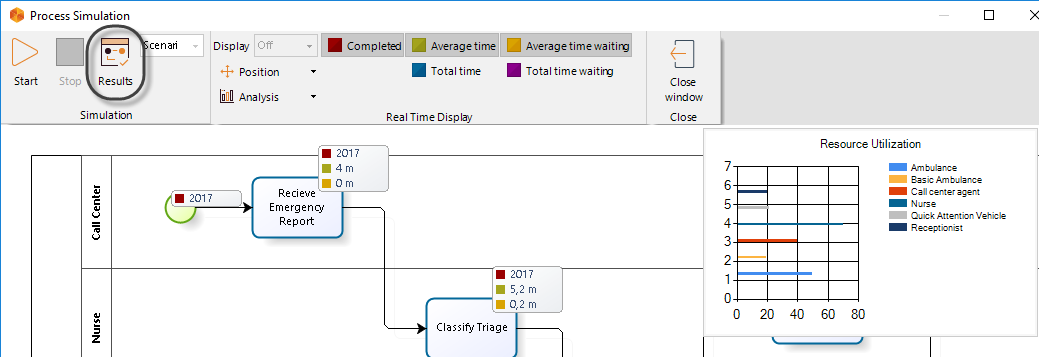
\includegraphics[width=10cm, keepaspectratio]{img/bizagi-process-simulation.png} }}%
    \qquad
    \subfloat{{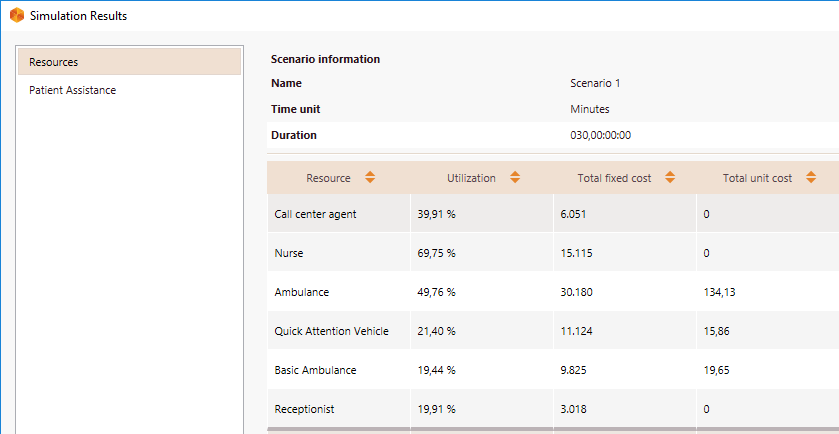
\includegraphics[width=10cm, keepaspectratio]{img/bizagi-simulation-results.png} }}%
    \caption{\textit{Bizagi Modeler} Resource analysis example\cite{bizagi-2018}}%
    \label{fig:bizagi-example}%
\end{figure}

% In this section a more details how \gls{bpms} works were provided. A two concrete solutions were shown and briefly described. These two systems became base inspiration for providing similar functionalities to \gls{bpms} based on DEMO (from now called \textit{Demo Machine}) . In the next section follows summarization, how DEMO Machine could work and how data could be aggregated and prepared to 
% visualisation.  

\section{DEMO Machine Based on BPMS}
As was told in introduction, thesis focuses mainly on fourth stage of \gls{bpm} life-cycle - a monitoring. However, to be able to visualise processes and collected data, some kind of process ``machine'' must be created. This ``machine'' must have ability to describe business processes or better, to model and run them. In other words, ``machine'' must support at least first three stages of life-cycle. In this thesis, details about this kind of ``machine'' are not provided. In introduction was mentioned work\cite{diploma-skotnica-2016} which is focused on creating and defining this kind of machine. Thesis uses knowledge about this DEMO Machine and assumes, that ``machine'' is created and behaves as is described from mentioned work.

\subsection{DEMO Machine Architecture}
Architecture of solution from  higher point of view can be described with \cref{fig:demo-machine-top}. This overview shows only main components (services) that are necessary to work. It is obvious, that every mentioned system must have many subsystems and dependencies (e.g. SQL databases, external resources,\dots). Each component can be described as:
\begin{figure}[ht!]
	\centering
    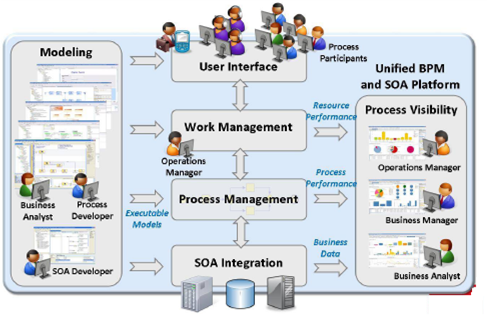
\includegraphics[width=12cm]{img/tibco-bpm-architecture.png}
    \caption{BPMS Architecture\cite{tibco-bpm-2016}}
    \label{fig:demo-machine-top}
\end{figure}
\begin{description}
	\item[Client Applications] They are client's specific systems and software within business. These applications are connected with \textit{Enterprise Service Bus}, which connects clients and \textit{DEMO Machine} together. It means, that done work within client's applications is projected to business processes inside \textit{DEMO Machine}.
    
    \item[Enterprise Service Bus] Data aggregation point where data from specific \textit{client's applications} are transformed to data that can be used within \textit{DEMO Machine}. Also it provides functionalities to provide data back from \textit{DEMO Machine} to clients.
	
    \item[DEMO Machine] The core system of whole solution. As was told earlier, \textit{DEMO Machine} supports at least first three stages of life-cycle (design, model, execute). Inside \textit{DEMO Machine} DEMO models (business processes) are defined along with actor roles. Into \textit{DEMO Machine} are connected external sources which use internal definitions of processes and machine is executing them. 
    
    \item[DEMO Machine Portal] Along side \textit{DEMO Machine} the portal serves to manage \textit{DEMO Machine}. Portal is divided to two sections:  
    
    \begin{enumerate}
    \item \textbf{Administration} section offers managing the \gls{demo} models. With graphical editors users can create \gls{ocd} diagrams, define actor roles and also create \gls{psd} diagrams and define \textit{Action rules}. Alongside designing models, inside administration users can assign actors (external users from client applications) to actor roles and manage running models.
    
    \item \textbf{Customer} section serves as end-user application which behaves according to defined processes. It has same behaviours and purpose as like many other \gls{bpms} solutions.
    \end{enumerate}
    
    \item[Data Aggregation Service] Another type of aggregation service. This time, collected data within defined processes inside \textit{DEMO Machine} are transformed a prepared for \textit{Business Intelligence Services}, which can be used for data visualisation.
    
    \item[Business Intelligence Services] Set of systems that provides \gls{bi} functionalities with interfaces to provide best overviews of precious collected data.   
\end{description}

Thesis focuses on ``Business Intelligence Services''. From Proposed approach is created proof-of-concept\footnote{Demonstration of concept. Its purpose is to verify that concept has potential for real-world usage\cite{proof-of-concept-2018}.} as mobile-application.

In this chapter, firstly more details about \gls{bpms} were provided. On the two concrete solutions available were taken the core concepts of process definitions and their visualisations. The \gls{bpms} solution based on DEMO was briefly described. High-level architecture overview of \textit{DEMO Machine} were explained. In the next chapter, visualisations of processes based on DEMO are described. 
